%%%%%%%%%%%%%%%%%%%%%%%%%%%%%%%%%%%%%%%%%%%%%%%%%%%%%%%%%%%%%%%%%%%%%%%%%%%
\chapter{Results}
%%%%%%%%%%%%%%%%%%%%%%%%%%%%%%%%%%%%%%%%%%%%%%%%%%%%%%%%%%%%%%%%%%%%%%%%%%%

The researcher conducted an experiment to validate the results
in \cite{Zaritsky2004}'s work. Following is the description of the 
experiment done.

The input strings used in the experiment were generated in a
 manner similar to the one used in DNA sequencing. That is, a random
string is generated, duplicated a predetermined number of times,
 and the copies are randomly divided into blocks of a given size. 
 The set of all these blocks is the input to the SCS problem. 
 The reasons for choosing this type of input has been extensively
 explained in \cite{Zaritsky2004}.
Since our random string is a sequence of characters \texttt{A},\texttt{C},\texttt{G}, and \texttt{T}, we must 
transform this into an equivalent binary string. To do this, we simply 
assign each letter a unique two-bit representation, that is, 
\texttt{A = 00}, \texttt{C = 01}, \texttt{G = 11}, and \texttt{T = 10}. 

The parameters used in the input generation is as follows:

\begin{tabular}{p{0.5cm}l}
&\textit{Size of random string}: 250 bases or characters\\
&\textit{Minimal block size}: 20 characters\\
&\textit{Maximal block size}: 30 characters\\
&\textit{Number of duplicates created from the random string}: 5\\
\end{tabular}

Let $l$ denote the length of the derived string in the
genetic algorithm case. Let $m$
denote the number of blocks not covered by the derived string, 
and let $b$ denote the maximal block size
(30, in our case). The fitness value, $f$ , of an individual
is computed as follows:
\[f = \dfrac{1}{l + m*b}\] 
This fitness function above drives evolution towards
shorter superstrings covering as many blocks as possible.

We performed 50 randomly generated problem instances.
On each problem instance each type of genetic algorithm was executed
twice and the better run of the two was used for statistical purpose.
The results are summarized in Table \ref{tbl:resultsga} and is presented graphically in Figure \ref{fig-results}.


\begin{table}
\centering
\begin{tabular}{|c|c|c|}
\hline
Number  & Average Superstring  & Average  \\
 of& Length (Rounded to & Runtime \\
Generations& Nearest Units) & (in Seconds) \\
\hline
\hline
100		& 760	& 34.57		\\
250		& 596	& 74.20		\\
500		& 526	& 139.70	\\
1000	& 482	& 267.09	\\
5000	& 421	& 1038.73	\\
10000	& 413	& 1943.55	\\
20000	& 409	& 3700.57	\\
\hline
\end{tabular}
\caption{
Average superstring length and runtime of our Genetic Algorithm
on 50 randomly generated problem instances. Each input set contains
50 blocks.}
\label{tbl:resultsga}
\end{table}


\begin{figure*}[ht!]
\centering
\fbox{
\scalebox{0.55}{
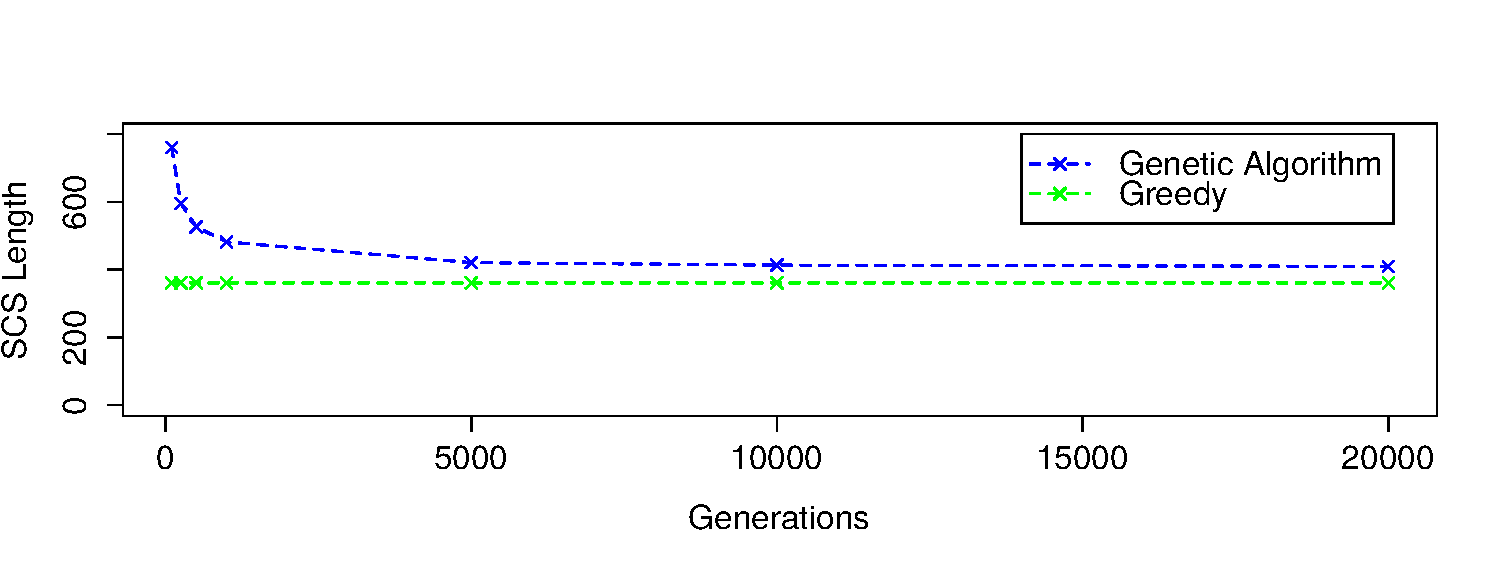
\includegraphics{result-gavsgreedy.pdf}
}}
\caption{Best superstring as a function of generations. Each point in the figure represents the average of 50
runs on 50 different randomly generated problem instances. For each such instance, two runs were performed, the better
of which was considered for statistical purposes}
\label{fig-results}
\end{figure*}

Note that our results seem to disagree with that of \cite{Zaritsky2004}.
In contrast with the latter's findings, our tests shows that
the greedy algorithm outperformed the genetic algorithm both in terms of finding superstrings
with minimal length and the the time it takes to do so.

On the same set of test cases, the greedy algorithm
produced superstrings having an average of 361 characters, 
in an average of runtime 130.64 milliseconds. This is far better than
the 409 average superstring length that the genetic algorithm
derived in 20000 generations in more or less an hour of operation. 
Note that the average length of the superstring derived by the greedy algorithm is
less than the conjectured factor-2 performance guarantee.
Recall that the length of the initial (reference) string is 250.

Still it is good to note that the genetic algorithm approach
in solving the SCS problem converges. That is, we see a better solution
yield as time or generations progress. 